




\section{Presentation of the competition}
\label{sec:competition}

	A company named \textit{Tradeshift} proposed a multi-label classification problem. 
	
	The input data provided represents elements of a text document and the objective of the competition is to classify those elements into 33 possible labels.
	In this chapter we'll start by defining what does the features of the input data consist of. We will then describe the labels provided. And will finish describing the evaluation criteria of this competition.


	\subsection{Input data}
	\label{sec:dataset}

		The competition relies on a dataset representing elements of text documents, we name it $X_o$. In \fref{fig:FeatureExtraction1}(a) you see a letter. For the competition this letter has been analyzed and many elements were taken out of it. The elements are shown on the \fref{fig:FeatureExtraction1}(b) as the red boxes and on (c) these elements are listed. In the competition, we see these elements as a 145 feature vector (namely $x_{o_i}$ with $i$ the sample index).

		\begin{figure}[h]
			\begin{center}
				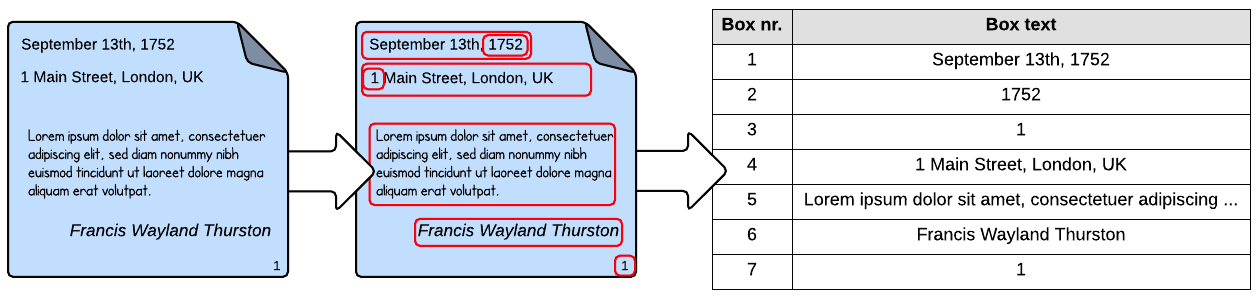
\includegraphics[width=0.9\textwidth]{FeatureExtraction1.png}
			\end{center}
			\caption{document segmentation from Kaggle website 
			\label{fig:FeatureExtraction1}}
		\end{figure}

		On \fref{fig:inputVector} you see The first 55 features of $x_{o_1}$. We don't know exactly what are the individual features, we just know what could they be. On the official description of the dataset \footnote{\url{http://https://www.kaggle.com/c/tradeshift-text-classification/details/evaluation}}, they say that a feature could either be a content feature, a parsing feature, a spatial feature or a relational features.

		\begin{itemize}
			\item "Content feature": is the direct representation of the text element in a hashed format.
			\item "Parsing feature": indicates which kind of characters are present on the text element. It can be for instance alphanumeric, numeric or text characters.
			\item "Spatial feature": is about position and size of the text element in the document.
		 	\item "Relational feature": gives information about the surrounding of our text element. If there is no values, it means the text element doesn't have a neighbor in that surrounding.
		\end{itemize}

		These features can be real valued, discrete valued, boolean valued or text valued. It can also happen that, for a given sample, the feature is \textit{no-valued}. This lack of value is represented by an empty string.

		I emphasize here that we still don't know what is on each of the individual features. Taking the example of feature number 1: we don't know what does this feature represent. Reading the file, we see that the feature 1 is either a YES, a NO or a no-value. But we can't say if it's a parsing feature, a spacial feature or a relational feature. We can just eliminate "content feature" as this feature is represented in a hash format.

		We can enjoy this last observation to assert that features 3, 4, 34, 35, 64, 65, 94, 95, 61 and 91 are content features as they all are hashed values (partially visible on \fref{fig:inputVector}).

	\subsection{Labels}
		The text elements just described represent something. For instance, the text elements seen on \fref{fig:FeatureExtraction1} represents a date, a number, an address, a text-body, a signature and a page number. In the competition we are given a vector of 33 labels for each of the text elements. That one can have one or more labels. For example an element could be labeled as a number and a page number. \Fref{fig:sample1_labels} is the label vector corresponding to the example seen above, where an extract of the 1st sample where shown on \fref{fig:inputVector}.

		As for the features, we don't know what a label correspond to. We are not given any names for the 33 label. We just have a number in the range from 1 to 33 as label.
		
		\begin{figure}
			\centering
			\begin{tabular}{ccccccccccccccccccccccccccccc}
				id & y1 & y2 & y3 & y4 & y5 & y6 & y7 & y8 & y9 & y10 & y11 \\ 
				1 & 0 & 0 & 0 & 0 & 0 & 0 & 0 & 0 & 0 & 0 & 0 \\
				\hline

				y12 & y13 & y14 & y15 & y16 & y17 & y18 & y19 & y20 & y21 & y22 & y23 \\
				0 & 0 & 0 & 0 & 0 & 0 & 0 & 0 & 0 & 0 & 0 & 0 \\
				\hline

				&y24 & y25 & y26 & y27 & y28 & y29 & y30 & y31 & y32 & y33 \\
				&0 & 0 & 0 & 0 & 0 & 0 & 0 & 0 & 0 & 1

			\end{tabular}
			\caption{Labels of sample with ID 1 given by \textit{Tradeshift}}
			\label{fig:sample1_labels}
		\end{figure}


	\subsubsection{files}
		All the data mentioned until now is provided through 3 csv files. 

		\begin{itemize}
			\item "train.csv": contains the training data $X_o$. It is an array of 1.7m lines of samples and 145 columns of features. Each cell has a either a real, a discrete, a boolean, a text value or a \textit{no-value}.
			\item "trainLabels.csv": contains label of data $Y$. It is an array of 1.7m lines of samples and 33 columns of labels. Each cell is either 0 or 1.
			\item "test.csv": contains the testing data. It is an array with merely 0.4m lines of samples and 145 columns of features. Each cell has a either a real, a discrete, a boolean, a text value or a \textit{no-value}.
		\end{itemize}



	\subsection{Evaluation criterion}
		The work is evaluated by sending a csv file on the \textit{kaggle} website. The csv file is then given a score by the system.

		That csv file has 2 columns and merely $33*0.4m=58$m lines. \Fref{fig:sample_prediction} is and example of this csv file. Each row of this file give an information about the pair \{sample $i$ and label $j$\}. The first column is a string encoding giving name this pair and the second column is the prediction corresponding to this same pair.

		\begin{figure}
			\centering
			\begin{tabular}{cc}
				id\_label & pred\\
				\hline

				1\_y1 & 0.01 \\
				1\_y2 & 0.05 \\
				1\_y3 & 0.98 \\
				2\_y1 & 0.1  \\
				2\_y2 & 0.88 \\
				2\_y3 & 0.92 \\

			\end{tabular}
			\caption{Prediction file of 2 samples with ID 1 and 2, and with 3 labels.}
			\label{fig:sample_prediction}
		\end{figure}


		Once submitted, the file receive a score through a scoring function. This function is the negative logarithm of the likelihood, averaged over $N_t$ test samples and $K$ labels.
		Mathematically, this function is defined as follows:

		\begin{equation} \label{eq1}
			\begin{split}
				LogLoss & = \frac{1}{N_t \cdot K} \sum_{idx=1}^{N_t \cdot K} LogLoss_{idx} \\
				&= \frac{1}{N_t \cdot K} \sum_{idx=1}^{N_t \cdot K} [-y_{idx} \log{\hat{y}_{idx}} - (1-y_{idx}) \log{(1-\hat{y}_{idx}) }] \\
		        &= \frac{1}{N_t \cdot K} \sum_{i=1}^{N_t} \sum_{j=1}^{K} [-y_{ij} \log{\hat{y}_{ij}} - (1-y_{ij}) \log{(1-\hat{y}_{ij}) }]
			\end{split}
		\end{equation}

		Where $\hat{y}_{idx}$ is the prediction of a sample for a given class and $y_{idx}$ is the true binary value stating if a sample belongs to a class or not.

		This function gives punishment for wrong confident predictions. 

		For instance, the LogLoss of one sample with one label predicting 0.001 instead of 1 (a confident wrong prediction) is $-\log(0.001) = 6.90776 $ whereas the log-loss of one sample with one label predicting 0.1 instead of 1 (a less confidently wrong prediction) is $-\log(0.1) = 2.30259$. As an indication, the LogLoss of predicting everything with $0.5$ probability is $-log(0.5) = 0.69315$ and the LogLoss of $0.95$ (for a $Y=1$) is $-\log(0.95) = 0.05129$


